\documentclass{article}

\usepackage{tikz}
\usepackage{pgfplots}
\usetikzlibrary{calc}
\usepackage{amsmath}
\usepackage{mathtools}
\usepackage{gensymb}
\usepackage{wrapfig}

\begin{document}
\section{Question A}

\section{Question B}
\begin{tikzpicture}
  \coordinate (a1) at (0,3);
  \coordinate (a2) at (1,2);
  \coordinate (a3) at (3,0);
  \coordinate (a4) at (6,3);
  \coordinate (a5) at (3,6);
  \coordinate (a6) at (-3,6);
  \coordinate (a7) at (-6,3);
  \coordinate (a8) at (-3,0);
  \coordinate (a9) at (-1,2);

  \draw[thick] (a1) to[out=0,in=90] (a2) to[out=-90, in=180] (a3) to[out=0, in=-90] (a4) to[out=90, in=0] (a5) -- (a6) to[out=180,in=90] (a7) to[out=-90,in=180] (a8) to[out=0,in=-90] (a9) to[out=90,in=180] cycle;
  \draw[thick, ->, magenta] (a1) --  ($(a1)-(0,1)$) node [below]{$a_{max}$};
  \draw[thick,|-|, red] (a5) -- node[midway, above]{a=0} (a6);
  \draw[thick, ->, cyan] (a7) -- ($(a7)-(0,2)$) node[below] {v};
  \draw[thick, ->, cyan] (a4) -- ($(a4)+(0,2)$) node[above] {v};
  \draw[thick, ->, cyan] (a8) -- ($(a8)+(2,0)$) node[below] {v};
  \draw[thick, ->, cyan] (a1) -- ($(a1)+(2,0)$) node[below] {v};
\end{tikzpicture}
Parts 1-3 are lablled on the picture.  For part 2, I was only looking for the flat portion, but inflection points are also places of a=0 (think about direction of acceleration, it changes.  This means there has to be a spot (inflection point) where a=0).

Part 4: There is no tangential acceleration!  Since there is no change in speed, there is no acceleration in the direction of the velocity, or tangent to the path, so there is no tangential velocity!

\section{Question C}
\begin{figure}[h]
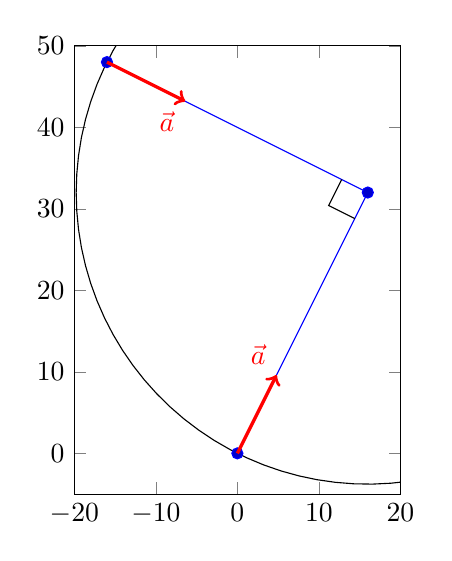
\begin{tikzpicture}
  \begin{axis}[xmin=-20, ymin=-5, ymax=50, xmax=20, axis equal image]
    \coordinate (start) at (axis cs:0,0);
    \coordinate (end) at (axis cs:-16,48);
    \coordinate (center) at (axis cs:16,32);
    \addplot coordinates{
      (0,0) (16,32) (-16,48)
    };
    \addplot[domain=-180:180, samples=100] ({16*sqrt(5)*cos(x)+16}, {16*sqrt(5)*sin(x)+32});
  \end{axis}
  \draw[very thick, ->, red] (start) -- ($0.7*(start)+0.3*(center)$) node[above left]{$\vec{a}$};
  \draw[very thick, ->, red] (end) -- ($0.7*(end)+0.3*(center)$) node[below left]{$\vec{a}$};
  \draw ($0.9*(center)+0.1*(end)$) -- ($0.8*(center)+0.1*(start)+0.1*(end)$) -- ($0.9*(center)+0.1*(start)$) ;
\end{tikzpicture}
\end{figure}
\begin{enumerate}
\item Look at picture
\item To solve this, we have to use a bit of geometry.  the accelerations both point towards the center of the circle, so they should both intersect at the center.  The equations of the lines are:
  \begin{gather*}
    y_1=2x_1 \\
    y_2 = -\frac{1}{2}x_2+40
  \end{gather*}
  (Verify these equations).  To find the center, we find where they intersect:
  \begin{gather*}
    2x = -\frac{1}{2}x+40 \\
    \frac{5}{2}x = 40 \\
    x = 16 \\
    \text{so\qquad} y = 2(16) = 32
  \end{gather*}
  From this, we get the radius of $16\sqrt{5}$ m using the Pythagorean Theorem.  Now, we have that our centripedal acceleration is below, so we can solve for velocity:
  \begin{gather*}
    a_c=\frac{v^2}{r} \\
    v=\sqrt{ar} \\
    v = \sqrt{(\sqrt{5})(16\sqrt{5})} = 4\sqrt{5} \text{ m/s}
  \end{gather*}
\item We find the period using our period equation, but first we need to find what fraction of the circle we travel around.  This is where a dot product is useful.  We want the angle between the two radii, so we do our dot product using our acceleration vectors:
  \begin{gather*}
    \begin{pmatrix}
      1\\2
    \end{pmatrix}
    \cdot
    \begin{pmatrix}
      2\\-1
    \end{pmatrix}
    = (1)(2)+(2)(-1)=0=|a|\:|b|\cos\theta \\
    \implies \theta = 90\degree
  \end{gather*}
  So our trip only happens around a fourth of the ring, so we just take a fourth of the period:
  \begin{gather*}
    \frac{T}{4} = \frac{1}{4}\frac{2\pi r}{v} = \frac{2\pi\: 16\sqrt{5}}{4(4\sqrt{5})}=2\pi\text{\:s}\approx 6.28\text{\:s}
  \end{gather*}
\item This problem has nothing to do with the previous section in the sense the times around the loop are the same!  Because the bike is starting from rest and changing its speed, the previous answers don't work! We have to use kinematic equations now if we want to find the new velocity:
  \begin{gather*}
    v_f^2=v_i^2+2a\Delta x \implies v_f=\sqrt{2a\Delta x}
  \end{gather*}
  We don't know the distance around the circle, but it is easy to find since it is just a fourth of the circumference!
  \begin{gather*}
    \Delta x = \frac{\text{Circumference}}{4} = \frac{2\pi(16\sqrt{5})}{4}=8\pi \text{\:m} \\
    v_f = \sqrt{2(0.5)(8pi)} \approx 7.50 \text{\:m/s}
  \end{gather*}
\item The total acceleration is the tangential acceleration plus the centripedal acceleration.  To find the magnitude, we need to add these values up, but they are perpendicular to each other, so all we need to do is take the Pythagorean sum
  \begin{gather*}
    |a_{tot}|=\sqrt{a_c^2+a_t^2}=\sqrt{ \left(\frac{v^2}{r}\right)^2+a_t^2}=\sqrt{ \left(\frac{(7.5)^2}{16\sqrt{5}}\right)^2+(0.5)^2}=1.65\text{\:m/s}^2
  \end{gather*}


  \begin{itemize}
  \item test
  \item ttest
  \end{itemize}
\end{enumerate}
\end{document}
